MedChain is developed in Go. Full Medchain code, its documentation as well as instructions on how to run it are available in \href{https://github.com/ldsec/medchain/tree/dev}{Medchain Github repository}. In this section, we aim to provide details about the code structure of MedChain node. We also provide instructions on how to setup and run MedChain node (i.e., server). In the end, we revisit MedChain query workflow, but this time in the context of its code and implementation.  
% Every MedChain node is a conode that offers certain funcitonalities defined as \textit{services}. 
% Full discussion of various server side code implementations

\subsection{MedChain API}
% Discussion of most important components of the API, how they function, and how they are used.
In this section, we provide details about some building blocks of MedChain Application Programming Interface (API). 

% \subsubsection{Authorization in MedChain}
% Give a general overview of how authorization is done in MedChain and what components are pivotal (with pointers to subsequent subsections)
\subsubsection{Smart Contract}
In Byzcoin, smart contract defines the data that is added to the ledger, i.e., data written to the ledger is, in fact, instances of smart contract. Also, smart contract gives us the API to manipulate the instances, for example, in order to create a new instance, we can \texttt{Spawn} an instance of smart contract and to update the contract instance, we can apply an \texttt{Invoke()} to it (this is explained in more details in \ref{background:byzcoin}). 

In MedChain, we define our own smart contract that implements the suitable data structure: the query. We developed the smart contract in Go (MedChain smart contract is located in \texttt{services} directory of the main code repository under the name \texttt{contract.go}). This smart contract is a simple key-value contract, meaning that every instance of the contract that is recorded in the ledger, i.e., the query, is a key-value store data structure. MedChain smart contract is identified by its name ``\textbf{MedChainContract}". This contract is distinguishable from any other contracts used in MedChain deployment such as Darc contracts (see Section \ref{lbl:darcs}) or Value contracts by its ID ``\textbf{MedChainContractID}". The client uses this ID in order to define which contract instance he/she wants to manipulate. The queries submitted to MedChain are recorded in the ledger as instances of \texttt{MedChainContract}. The structure of these queries is shown in Figure \ref{fig:medchain_query}. 

In ByzCoin, it is mandatory that the smart contract implement three API methods: \texttt{Spawn}, \texttt{Invoke}, and \texttt{Delete}. The very first instance of a contract is created by creating a transaction using \texttt{Spawn} as the instruction. By this transaction, the user sets the query ID as the key of the instance and its status as the value. Later, the user can manipulate this instance of the contract by calling an \texttt{Invoke} on it. The \texttt{Invoke} method in \texttt{MedChainContract} implements two methods itself: \texttt{update} and \texttt{verifystatus}. Using update, the user is able to retrieve a specific contract instance (i.e., query) from the Skipchain by its key (i.e., query ID) and update its value (i.e., the status of the query) if it already exists in the skipchain, however, if that is not the case, a new instance of the contract will be spawned using the provided key-value pair. \texttt{verifystatus} method is used by MedChain node itself to retrieve a query from the ledger and verify its status in a similar manner to \texttt{update} method. In MedChain, we decided not to implement the \texttt{Delete} function in contract as we do not want the user to be able to remove a query (i.e., an instance of the contract) from the global state. 

Whenever a contract instance is created (spawned) it is allocated an \texttt{InstanceID} that is determined based on the ID of the Darc contract ruling it. Later, this instance of the contract is retrievable and authorized by the Darc controlling it using this \texttt{InstanceID}.

\subsubsection{Deferred Transaction}
In order to enable multi-signature rules in MedChain, we use ByzCoin \textit{deferred transactions}. Deferred transactions allow a transaction to remain \textbf{proposed} (i.e., not written to the ledger) until it receives the threshold number of signatures defined by the Darc governing it. Once it receives enough number of signatures, it can be \textbf{executed} and written to the ledger. 

In order to enable deferred transactions in ByzCoin server, the developer should define a special method in the smart contract, namely, \texttt{VerifyDeferredInstruction}, which is not implemented in a \texttt{BasicContract} (i.e., the basic data structure that all contracts implement by default). In other words, types which embed \texttt{BasicContract} must override this method if they want to support deferred transactions (using the \texttt{Deferred contract}). 

To enable deferred execution of a \texttt{MedChainContract} instance, the following steps are taken:
\begin{enumerate}
    \item User spawns a \texttt{MedChainContract} instance (this is the proposed transaction).
    \item User spawns a \texttt{deferred\_contract} instance with query instance ID as its arguments. In other words, the proposed transaction is the what the deferred instance holds.
    \item Signers sign the proposed transaction by invoking an \texttt{addProof} on the corresponding deferred instance.
    \item User invokes an \texttt{execProposedTx} on the corresponding deferred instance to execute the proposed transaction.
\end{enumerate}

It is important to note that ByzCoin does not perform any checks on the signatures added during \texttt{addProof} transaction. This means that even garbage signatures can be added to the deferred transactions (but still adding the same signature multiple times is not permitted). However, the signatures and Darc rules are checked during \texttt{execProposedTx} transactions. In MedChain, only a maximum of one execution is allowed per proposed query transaction and extra executions are rejected. 

\subsubsection{Darcs (Distributed Access Right Controls)} \label{lbl:darcs}
Darcs are used to enable authorization in MedChain. In ByzCoin, Darcs are responsible for handling authorization and access management for various resources, such as smart contract instances, and they use action/expression pairs to define rules.

ByzCoin offers some Darcs in its \texttt{darc} library such as \texttt{SecureDarc}, however, the developer can also develop his/her own Darc contract. In MedChain, we use \texttt{SecureContract} and have customized it to meet the requirements of MedChain. 

\texttt{SecureDarc} contract defines access rules for all clients using Darc data structure. Upon starting a network of MedChain servers, a new ByzCoin blockchain and a \texttt{genesis Darc} instance are created. The \texttt{genesis Darc} indicates what instructions need which signatures to be accepted. Below, you can see how the \texttt{genesis Darc} we use in MedChain looks like:

\begin{verbatim}

- Darc:
    -- Description: "genesis darc"
    -- BaseID: darc:<ID_genesis_darc>
    -- PrevID: darc:<ID_darc>
    -- Version: 0
    -- Rules:
        --- invoke:config.update_config - "ed25519:<ID_client>"
        --- spawn:darc - "ed25519:<ID_client>"
        --- invoke:darc.evolve - "ed25519:<ID_client>"
        --- invoke:darc.evolve_unrestricted - "ed25519:<ID_client>"
        --- _sign - "ed25519:3<ID_client>"
        --- spawn:naming - "ed25519:<ID_client>"
        --- spawn:MedChainContract - "ed25519:<ID_client>"
        --- invoke:MedChainContract.update - "ed25519:<ID_client>"
        --- invoke:MedChainContract.verifystatus - "ed25519:<ID_client>"
        --- _name:MedChainContract - "ed25519:<ID_client>"
        --- invoke:config.view_change - "ed25519:<ID_server> 
            | ed25519:<ID_server> | ed25519:<ID_server>"
    -- Signatures:
    
\end{verbatim}

In the above \texttt{genesis Darc}, we can see the pairs of \texttt{action/expression} that define different rules. For example, \texttt{spawn:MedChainContract - "ed25519:<ID\_client>"} where \texttt{ID\_client} refers to the ID of the client who is granted the permission for the action \texttt{spawn:MedChainContract} which in this case is the ByzCoin admin. Darc expressions are a simple language for defining complex policies. For example, in the rule \texttt{invoke:config.view\_change - "ed25519:<ID\_server> | ed25519:<ID\_server>"}, an ``\texttt{or}" expression has been used among the IDs of MedChain cluster servers. 

As we mentioned earlier, in MedChain, projects define various databases and in order to control access to the database, every project is associated with a Darc. Here, we consider the example of having \texttt{Project A} and \texttt{Project B} and a cluster of 3 MedChain nodes. We create Darcs for each of these projects. We assume that each project has 3 clients (i.e., one client per MedChain node). We create new Darcs and define rules (i.e., action/expression pairs) for them. As an example, the Darc for project A is given below:

\begin{verbatim}
- Darc:
    -- Description: "Project A Darc"
    -- BaseID: darc:<ID_darcA>
    -- PrevID: darc:<ID_genesis_darc>
    -- Version: 0
    -- Rules:
        --- _evolve - "ed25519:<ID_owner>" 
        --- _sign - "ed25519:<ID_client1>" | 
        "ed25519:<ID_client2>" | "ed25519:<ID_client3>"
        --- spawn:MedChainContract - "ed25519:<ID_client1>" | 
        "ed25519:<ID_client2>" | "ed25519:<ID_client3>"
        --- invoke:MedChainContract.update - 
        "ed25519:<ID_client1>" | "ed25519:<ID_client2>" |
        "ed25519:<ID_client3>"
        --- invoke:MedChainContract.patient_list - 
        "ed25519:<ID_client1>" | "ed25519:<ID_client2>" |
        "ed25519:<ID_client3>"
        --- invoke:MedChainContract.count_per_site - 
        "ed25519:<ID_client1>" | "ed25519:<ID_client2>" 
        | "ed25519:<ID_client3>"
        --- invoke:MedChainContract.count_per_site_obfuscated - 
        "ed25519:<ID_client1>" | "ed25519:<ID_client2>" | 
        "ed25519:<ID_client3>"
        --- invoke:MedChainContract.count_per_site_shuffled - 
        "ed25519:<ID_client1>" | "ed25519:<ID_client2>" |
        "ed25519:<ID_client3>"
        --- invoke:MedChainContract.count_per_site_shuffled_obfuscated - 
        "ed25519:<ID_client1>" 
        --- invoke:MedChainContract.count_global - 
        "ed25519:<ID_client1>" 
        --- invoke:MedChainContract.count_global_obfuscated - 
        "ed25519:<ID_client1>" 
    -- Signatures:
\end{verbatim}

In the above Darc for \texttt{Project A}, we have defined rules using different types of actions and expressions. For example, all users can take action  \texttt{invoke:MedChainContract.patient\_list} and in order for it to be approved, the signature of \textbf{any} of the signers is enough as an \texttt{OR} expression is used among signer identities. However, only client 1 is given permission to query \texttt{count\_global} from database A (i.e., the action \texttt{invoke:MedChainContract.count\_global}). 

Now, let's see how the Darc for \texttt{Project A} can authorize an action. The first step is that the client sends a spawn instruction to \texttt{Project A} Darc contract. Then, the client asks the instance to create a new instance with the \texttt{MedChainContractID} of MedChain smart contract, i.e., \texttt{MedChainContract}, which is different from the ID of the Darc instance itself. The client must be able to authenticate against a \texttt{spawn:MedChainContract} rule defined in the Project A Darc instance which is indeed the case according to Project A Darc definition above. The transaction that client creates looks like below:

\begin{verbatim}
instr := byzcoin.Instruction{
    InstanceID: byzcoin.NewInstanceID(<Project A Darc ID>),
    Spawn: &byzcoin.Spawn{
    ContractID: "MedChainContract",
    Args: byzcoin.Arguments{
		    {
		        Name:  < query ID including the action>,
		        Value: []byte("Submitted"), 
		    },
        }  
    },
    SignerCounter: c.nextCtrs(),
}
\end{verbatim}

The new instance spawned will have an instance ID equal to the hash of the Spawn instruction. This instance ID is the hook to this instance and the client needs to remember this it in order to manipulate this instance later, for example, invoke methods on it to update its status. In MedChain, we also use \texttt{contract\_name} of ByzCoin. This contract is a singleton contract that is always created in the genesis block. One can only invoke the \texttt{naming contract} to relate a Darc ID and name tuple to another instance ID. Once an instance is named, the client can the name given to the instance ID to retrieve it from the ledger.

After this step, a \texttt{MedChainContract} instance spawned by the user (which is in fact the query submitted to MedChain from MedCo-connector) is bound to Project A Darc and is governed by it; thus, the Darc can check for the authorizations of the action the client is trying to take.

Important point: since the very first transaction, i.e., the one created right after MedChain receives a query from MedCo, is always immediately written to the ledger (due to auditability purposes) using a \texttt{Spawn} instruction of \texttt{Value} contract, all project Darcs need to have \texttt{spawn:value} and \texttt{invoke:value} rules enabled for all Darc users (i.e., using an \textit{at least one} expression).


\subsection{MedChain Service}
% Explanation of what MedChain service does, how it interacts with the API and handles requests and responds to them.  
In Cothority, every app (e.g. Command-Line-Interface app) or client (at the front-end) communicates with services to interact with Conodes. In other words, services are responsible for handling Client-to-Conode communications. Services are based on \href{https://github.com/dedis/onet}{Onet library} that provides the overlay network and enables definition of communication protocols in Cothority. A service is created with Conode. It serves client requests, creates protocols for Overlay network (see later), and handles communication of the information to other services on other Conodes. 

In MedChain node implementation, in order to define client-MedChain node communications and enable message sharing among them, we defined our own service. MedChain service code can be found in \texttt{services/service.go} in the main code repository. In MedChain service, that is based on Onet, we define services that use Protocols which can send and receive messages. This means that MedChain node uses Onet to send/receive messages to/from the client over the service-API, which is implemented using protobuf over WebSockets. Messages defined in MedChain are explained in next section.


\subsubsection{MedChain Messages and API Calls}
% Explanation of messages and calls defined in MedChain, both in words and using a table. 
In MedChain, we mainly used two services: ByzCoin and Onet services that enable client-server communications. We define Medchain API using these services and later implement the CLI-program on top of this API (see Section \ref{section5}). Messages defined and used in MedChain can be found in \texttt{services/struct.go} in code repository. Table \ref{tbl:med_api_calls} shows some of the most important messages defined in MedChain as well as resources they take and their responses.

\begin{table}[ht]
\centering
\caption{Most Important Medchain API calls}
\label{tbl:med_api_calls}
\begin{tabular}{|l|l|l|l|}
\hline
\textbf{Name of Method} & \textbf{Description} & \textbf{Resources} & \textbf{Response}\\
\hline
\\[-1em]
\textbf{AddQuery}    &  Spawn a query transaction& \pbox{20cm}{ User ID,\\ Query definition, \\ Darc ID \\[1pt]}  & \pbox{20cm}{Instance ID, \\ OK? }\\ 
\hline
\\[-1em]
\textbf{AddDeferredQuery} & Spawn a deferred query transaction  &  \pbox{20cm}{ User ID, \\ Query definition, \\ Instance ID, \\ Darc ID \\[1pt]}  & \pbox{20cm}{Instance ID, \\ OK? } \\
\hline
\\[-1em]
\textbf{SignDeferredTx} & Sign a deferred query transaction  & \pbox{20cm}{ User ID,\\ User keys, \\ Instance ID \\[1pt]} & \pbox{20cm}{Instance ID, \\ OK? } \\
\hline
\\[-1em]
\textbf{ExecDeferredTx} & Execute a deferred query transaction  & \pbox{20cm}{ User ID,\\ Instance ID, \\[1pt]} & \pbox{20cm}{Instance ID, \\ OK? } \\
\hline
\\[-1em]
\textbf{AuthorizeQuery} & Authorize a query  & \pbox{20cm}{ Query definition,\\ Instance ID, \\ Darc ID\\[1pt]} & \pbox{20cm}{Instance ID, \\ Query Status,\\ OK? } \\
\hline
\\[-1em]
\textbf{GetSharedData} & Get instance IDs shared with node  & \pbox{20cm}{ - } & \pbox{20cm}{Instance IDs } \\
\hline
 \\[-1em]
\textbf{PropageteID} & Broadcast instance IDs to roster& \pbox{20cm}{ Instance ID,\\ Roster \\ } & \pbox{20cm}{OK? } \\
\hline
\end{tabular}
\end{table}


\subsection{MedChain Protocol}
% Discussion of what is a protocol, why it is used, and how MedChain protocol works. 
In Cothority, protocols are responsible for handling Conode-to-Conode communications. In MedChain, we use the protocol defined in MedCo-unlynx which can be found in \texttt{protocols} directory of MedChain repository. The protocol is instantiated with service whenever needed and is used to broadcast the instance ID of deferred transactions to all MedChain nodes in the roster. 

Both services' and protocols' binaries loaded into MedChain node at compile time using package imports as it can be seen in main server code found in file  \texttt{cmd/medchain-server/medchain.go}. 


\subsection{MedChain Node}
% i.e., developing MedChain App in order to make services available in MedChain nodes and to be able to use CLI to interact with server.
MedChain node is a Conode that has specific MedChain services and protocols available in it. The main MedChain node (i.e., server) code can be found \texttt{cmd/medchain-server}. Table \ref{tbl:server_cmds} shows the commands (subcommands of \texttt{server}) that are supported in MedChain node.  

\begin{table}[ht]
\centering
\caption{MedChain Server:\texttt{server} command and its subcommands }
\label{tbl:server_cmds}
\begin{tabular}{|l|l|l|}
\hline
\textbf{Command} & \textbf{Description} & \textbf{Arguments}\\
\hline
\\[-1em]
\textbf{\texttt{server}}    &  Run MedChain server & \pbox{20cm}{\texttt{--c}: Server configuration file \\ \texttt{--d}: debug-level\\[1pt]}\\
\hline
\\[-1em]
\textbf{\texttt{server setup}}    &  Setup MedChain server & -\\
\hline
\\[-1em]
\textbf{\texttt{server setupNonInteractive}} & Setup server non-interactively  &  \pbox{20cm}{\texttt{--sb}: server binding \\ \texttt{--desc}: node description \\ \texttt{--priv}: Private toml file path \\ \texttt{--pub}: Public toml file path \\ \texttt{--privKey}: Provided private key \\ \texttt{--pubKey}: Provided public key \\[1pt]}\\
\hline
\\[-1em]
\textbf{\texttt{server config}} & Check servers in roster  & \pbox{20cm}{\texttt{--g}: Group definition file \\ \texttt{--t}: Set a different timeout\\[1pt]} \\
\hline
\end{tabular}
\end{table}


\subsubsection{MedChain Node: Setup and Run}
The easiest way to setup and run multiple MedChain nodes (locally and as a shell process) is to use the provided shell script \texttt{run\_nodes.sh} at \texttt{/cmd/medchain-server/} directory of MedChain repository. For example, the following code can be executed in order to run 3 MedChain nodes:
\begin{verbatim}
    path/to/medchain/cmd/medchain-server$ go build
    path/to/medchain/cmd/medchain-server$ run_nodes.sh -n 3 -d medchain-config
\end{verbatim}

The above code, will setup and start 3 MedChain nodes and will put all configuration files in \texttt{./medchain-config/}. The file containing public configurations will be in \texttt{./medchain-config/group.toml}. The folders created in \texttt{./medchain-config/} (i.e., \texttt{mc1/}, \texttt{mc2/}, ...) each hold private keys of a server in \texttt{private.toml}. The servers will then be listening to ports. It is important to note that each MedChain node uses two ports. MedChain-to-MedChain communication is automatically secured via TLS when you use the unchanged configuration from MedChain server setup. However, MedChain-to-client communication happens on the next port up from MedChain-to-MedChain port and it defaults to WebSockets inside of HTTP.

Additionally, it is possible to run MedChain nodes one at a time and without the mentioned script. To this end, the command below can be used to run a single MedChain node:
\begin{verbatim}
    path/to/medchain/cmd/medchain-server$ go build
    path/to/medchain/cmd/medchain-server$ ./medchain-server server setup
    path/to/medchain/cmd/medchain-server$ ./medchain-server server setup
\end{verbatim}

After the above commands are run, MedChain node is setup. Now, to run the server, the following can be used:
\begin{verbatim}
    path/to/medchain/cmd/medchain-server$ ./medchain-server server setup
    path/to/medchain/cmd/medchain-server$ ./medchain-server server
\end{verbatim}


Last but not least, one can use Docker to run a single MedChain server or a network of them. This is explained in details in Section \ref{section6}.  

\subsection{MedChain Query Workflow Revisited} \label{workflow-revisited}
Now that we have described and discussed the implementation of a MedChain node, we can consider its query workflow with a code and implementation perspective. 
Figure \ref{fig:medchain_full_flow}, illustrates various code components of MedChain, operations that happen in MedChain, the interfaces, as well as communications in MedChain. As it is shown in this figure, in the front end, we have the CLI (Command-Line-Interface) client, (see Section \ref{section5} for further details) and the Go API client, explained earlier in the section, that interact with MedChain node by sending requests to it. In the back end, MedChain node, also a member of MedChain network, serves the client requests. The steps below explain detailed query workflow in MedChain and correspond to numbered operations in Figure \ref{fig:medchain_full_flow}:

\begin{enumerate}
    \item CLI client submits a query to MedChain Go API client for authorization through a client call. The query has the structure shown in Figure \ref{fig:medchain_query}. 
    
    \item Go API client sends the query to MedChain node for authorization per service call. Then, the transaction to spawn the Value contract (that implements a simple key-value pair) instance is \textbf{prepared} with the query ID as its key and query status \texttt{Submitted} as its value. Please note that the query ID contains what the actual user query is (e.g., patient\_list, etc.) and that is the \textbf{action} which is authorized or rejected. See Section \ref{arch:flow} and Figure \ref{fig:medchain_query}. 
    
    \item MedChain looks up the Darc governing the query to check the authorizations for the action. 
    
    
    \item Depending on the Darc rule, the action is either rejected/authorized. Then, the transaction is executed and the status of value query instance is updated correspondingly. Finally, the result is written to ledger after ByzCoin nodes achieve consensus. 
    
    \item The status of query is sent back to client through a service call. If the status is \texttt{Rejected}, the process stops here. 
    
    \item If the query is authorized, Go API sends a request to spawn an instance of MedChain contract through a service call. Its key is the query ID and the status of query is not relevant in this step. A transaction containing the query ID and status (=empty) is created. 
    
    \item An instance of deferred contract is \textbf{spawned} with the transaction in previous step as its \textbf{proposed transaction}. The instance ID of this deferred contract instance is broadcast to all MedChain nodes in the network using MedChain protocol so that their clients can later use this instance ID to sign the proposed transaction.
    
    \item Client sends request to sign the proposed transaction to Go API client. The request contains the instance ID of targeted deferred instance.  
    
    \item Go API client invokes an \texttt{addProof} on the deferred contract instance holding the proposed transaction in order to sign it.
    
    \item Client sends request to execute the proposed transaction to Go API client. The request contains the instance ID of targeted deferred instance.
     
    \item Go API client invokes an \texttt{execProposedtx} on the deferred contract instance holding the proposed transaction in order to execute it. 
    
    
    
    \item Provided that enough signatures have been already added to the proposed transaction, it is executed and it is added to the blockchain with status \texttt{Authorized}.
    
\end{enumerate}

\begin{figure}[htbp] 
        \centering 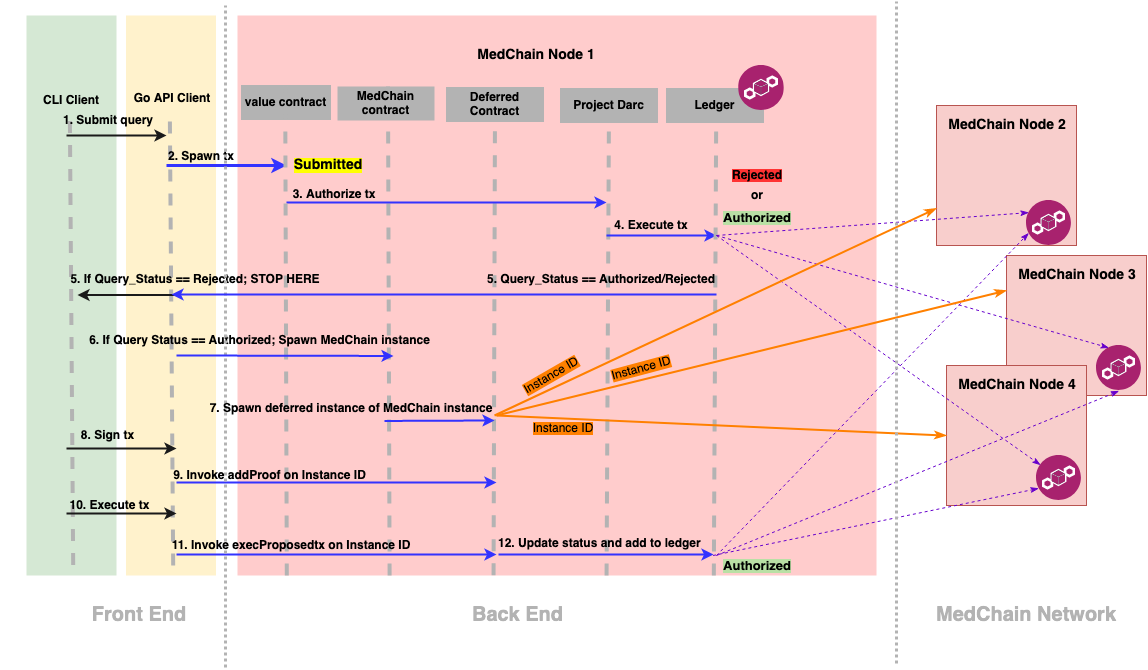
\includegraphics[width=1\columnwidth]{Images/full-flow-presentation.png}
        \caption{\label{fig:medchain_full_flow} 
         Detailed workflow of queries in MedChain with respect to various code components. In this figure, black arrows show client calls, blue arrows represent MedChain service calls (client-to-MedChain communications), orange arrows show communications handled by the protocol (MedChain-to-MedChain communications), and dashed arrows correspond to ByzCoin-to-ByzCoin communications.
        }
\end{figure}


% % Every Medchain node is a cothority server, known as a conode. There are several ways to initialize a conode that are described in conode documentation found at \cite{conode:2019}. In this project, we used \href{https://github.com/dedis/cothority/blob/master/conode/README.md#option-1-computer-configuration-setup-with-the-command-line}{configuration setup with the command line} to setup our network of 3 local conodes in an interactive manner. Also, in order to use the conodes we followed the instructions to \href{https://github.com/dedis/cothority/blob/master/conode/README.md#option-1-computer-run-with-the-command-line}{run} them. 

% The main point to note here is that once a smart contract is developed and imported into a conode, it is available and can be used by the client. This means that the user does not need to bootstrap the smart contract or install it.  

% \subsection{API}
% In this section, we provide details about some building blocks of the Medchain Application Programming Interface (API). 

% \subsubsection{Smart Contract} \label{impl:smart_contract}
% The smart contract provides the user with the API to interact with the skipchain (i.e., the ledger) by adding, updating, or removing the instances of the contract from the ledger. 

% We developed the smart contract in Go using the template contract provided in cothority\_template repository called  \href{https://github.com/dedis/cothority_template/tree/master/byzcoin}{ByzCoin example} which is a simple key-value contract, meaning that every instance of the contract that is recorded in the ledger is a key-value store data structure. Medchain smart contract is identified by its name "\textbf{queryContract}". This contract is distinguishable from any other contract used in Medchain deployment such as Darc contracts (see Section \ref{impl:darcs}). The client uses this ID in order to define which contract instance he/she wants to manipulate. The queries submitted to Medchain are recorded in the ledger as instances of \texttt{queryContract}. The structure of these queries is shown below: 

% \begin{verbatim}
% type Query struct {
% 	    ID     string //<query_id>:<user_id:databaseX>:<type of query>
% 	    Status string // "Submitted", "Authorized", or "Rejected"
% } 
% \end{verbatim}

% As it is shown above, the key of a queryContract instance is the ID of the query and the value is its status.  

% To serve the purposes of Medchain, we changed some functionalities of the template contract so that it is adapted to Medchain ecosystem. In ByzCoin, the smart contract has to implement three API methods: \texttt{Spawn},\texttt{Invoke}, and \texttt{Delete}. The very first instance of a contract is created by creating a transaction using \texttt{Spawn} as the instruction. By this transaction, the user sets the query ID as the key of the instance and its status as the value. Later, the user can manipulate this instance of the contract by calling an \texttt{Invoke} on it. The \texttt{Invoke} method in \texttt{queryContract} implements two methods itself: \texttt{update} and \texttt{verifystatus}. Using update, the user is able to retrieve a specific contract instance (i.e., query) from the skipchain by its key (i.e., query ID) and update its value (i.e., the status of the query) if it already exists in the skipchain, however, if that is not the case, a new instance of the contract will be spawned using the provided key-value pair. \texttt{verifystatus} method is used by Medchain server itself to retrieve a query from the ledger and verify its status in a similar manner to \texttt{update} method. In Medchain, we decided not to implement the \texttt{Delete} function in contract as we do not want the user to be able to remove a query (i.e., an instance of the contract) from the global state. 

% Whenever a contract instance is created (spawned) it is allocated an \texttt{InstanceID} that is based on the ID of the Darc contract governing it (please refer to Section \ref{background:smart_contract} for more details). Later, this instance of the contract is retrievable and authorized by the Darc controlling it using this \texttt{InstanceID}. 

% \subsubsection{Deferred Transactions} \label{impl:deferred_tx}
% In a real world scenario, it is not always possible for hospitals (running Medchain servers) to approve queries they receive from other Medchain servers instantly, for example, the hospital manager may not be present or the local Medchain server may be down. Thus, the query will be rejected as it will not receive the threshold number of signatures from other Medchain servers in the network it needs so that it is deemed as approved at the time it is created. There should be a mechanism in Medchain to handle this issue. \textbf{Deferred transactions} can be used as a solution for this problem. As the name suggests, deferred transactions allow a transaction to remain idle until it receives the threshold number of signatures it needs to be written in the ledger.  

% In order to enable deferred transactions in ByzCoin server, the developer should define a special method in the smart contract, namely, \texttt{VerifyDeferredInstruction}, which is not implemented in a \texttt{BasicContract} (i.e., the basic data structure that all contracts implement by default). In other words, types which embed \texttt{BasicContract} must override this method if they want to support deferred transactions (using the \texttt{Deferred contract}). 

% To enable deferred execution of a \texttt{queryContract} instance, the following steps are taken:
% \begin{enumerate}
%     \item User spawns a \texttt{queryContract} instance (This is the proposed transaction).
%     \item User spawns a \texttt{deferred\_contract} instance with query instance as its arguments.
%     \item Signers sign the proposed transaction and invoke an \texttt{addProof} on it.
%     \item User invokes an \texttt{execProposedTx} on proposed transaction to execute it.
% \end{enumerate}

% \subsubsection{Darcs} \label{impl:darcs}
% In ByzCoin, Darcs are used to enable authorization and access management and are, in fact, smart contracts. The only difference between a Darc and a general smart contract is that a Darc supports \texttt{actions} and \texttt{expressions} that are used to define a set of rules in a Darc.

% ByzCoin offers some Darcs in its \texttt{darc} library such as \texttt{SecureDarc}, however, the developer can also develop his/her own Darc contract. In Medchain, we use \texttt{SecureContract} and have customized it to meet the requirements of Medchain. 

% \texttt{SecureDarc} contract defines access rules for all clients using the Darc data structure. Upon starting a cluster of Medchain servers, a new ByzCoin blockchain and a \texttt{genesis Darc} instance are created. The \texttt{genesis Darc} indicates what instructions need which signatures to be accepted. Below, you can see how the \texttt{genesis Darc} we use in Medchain looks like:

% \begin{verbatim}

% - Darc:
%     -- Description: "genesis darc"
%     -- BaseID: darc:<ID_genesis_darc>
%     -- PrevID: darc:<ID_darc>
%     -- Version: 0
%     -- Rules:
%         --- invoke:config.update_config - "ed25519:<ID_client>"
%         --- spawn:darc - "ed25519:<ID_client>"
%         --- invoke:darc.evolve - "ed25519:<ID_client>"
%         --- invoke:darc.evolve_unrestricted - "ed25519:<ID_client>"
%         --- _sign - "ed25519:3<ID_client>"
%         --- spawn:naming - "ed25519:<ID_client>"
%         --- spawn:queryContract - "ed25519:<ID_client>"
%         --- invoke:queryContract.update - "ed25519:<ID_client>"
%         --- invoke:queryContract.verifystatus - "ed25519:<ID_client>"
%         --- _name:queryContract - "ed25519:<ID_client>"
%         --- invoke:config.view_change - "ed25519:<ID_server> 
%             | ed25519:<ID_server> | ed25519:<ID_server>"
%     -- Signatures:
    
% \end{verbatim}

% In the above \texttt{genesis Darc}, we can see the pairs of \texttt{action/expression} that define different rules. For example, \texttt{spawn:queryContract - "ed25519:<ID\_client>"} where \texttt{ID\_client} refers to the ID of the client who is granted the permission for the action \texttt{spawn:queryContract}. Darc expressions are a simple language for defining complex policies. For example, in the rule \texttt{invoke:config.view\_change - "ed25519:<ID\_server> | ed25519:<ID\_server>"}, an "\texttt{or}" expression has been used among the IDs of Medchain cluster servers. 

% Now, we create Darcs for different projects (e.g., \texttt{Project A} and \texttt{Prject B}) in Medchain. We assume that each project has 3 clients (i.e., one client per Medchain server). We create new Darcs and define rules (i.e., action/expression pairs) for them. As an example, the Darc for project A is given below:

% \begin{verbatim}
% - Darc:
%     -- Description: "Project A Darc"
%     -- BaseID: darc:<ID_darcA>
%     -- PrevID: darc:<ID_genesis_darc>
%     -- Version: 0
%     -- Rules:
%         --- _evolve - "ed25519:<ID_owner>" 
%         --- _sign - "ed25519:<ID_client1>" | 
%         "ed25519:<ID_client2>" | "ed25519:<ID_client3>"
%         --- spawn:queryContract - "ed25519:<ID_client1>" | 
%         "ed25519:<ID_client2>" | "ed25519:<ID_client3>"
%         --- invoke:queryContract.update - 
%         "ed25519:<ID_client1>" | "ed25519:<ID_client2>" |
%         "ed25519:<ID_client3>"
%         --- invoke:queryContract.patient_list - 
%         "ed25519:<ID_client1>" | "ed25519:<ID_client2>" |
%         "ed25519:<ID_client3>"
%         --- invoke:queryContract.count_per_site - 
%         "ed25519:<ID_client1>" | "ed25519:<ID_client2>" 
%         | "ed25519:<ID_client3>"
%         --- invoke:queryContract.count_per_site_obfuscated - 
%         "ed25519:<ID_client1>" | "ed25519:<ID_client2>" | 
%         "ed25519:<ID_client3>"
%         --- invoke:queryContract.count_per_site_shuffled - 
%         "ed25519:<ID_client1>" | "ed25519:<ID_client2>" |
%         "ed25519:<ID_client3>"
%         --- invoke:queryContract.count_per_site_shuffled_obfuscated - 
%         "ed25519:<ID_client1>" 
%         --- invoke:queryContract.count_global - 
%         "ed25519:<ID_client1>" 
%         --- invoke:queryContract.count_global_obfuscated - 
%         "ed25519:<ID_client1>" 
%     -- Signatures:
% \end{verbatim}

% In the above Darc for Project A, we have defined rules using different types of actions and expressions. For example, all users can take action  \texttt{invoke:queryContract.patient\_list} and in order for it to be approved, the signature of \textbf{any} of the signers is enough as an \texttt{OR} expression is used among signers. However, only client 1 is given permission to query \texttt{count\_global} from database A (i.e., the action \texttt{invoke:queryContract.count\_global}). 

% Now, let's see how the Darc for Project A can authorize an action. The first step is that the client sends a spawn instruction to Project A Darc contract. Then, the client asks the instance to create a new instance with the \texttt{contractID} of Medchain smart contract, i.e., \texttt{queryContract}, which is different from the ID of the Darc instance itself. The client must be able to authenticate against a \texttt{spawn:queryContract} rule defined in the Project A Darc instance which is indeed the case according to Project A Darc definition above. The transaction that client creates looks like below:

% \begin{verbatim}
% instr := byzcoin.Instruction{
%     InstanceID: byzcoin.NewInstanceID(<Project A Darc ID>),
%     Spawn: &byzcoin.Spawn{
%     ContractID: "queryContract",
%     Args: byzcoin.Arguments{
% 		    {
% 		        Name:  < query ID including the action>,
% 		        Value: []byte("Submitted"), 
% 		    },
%         }  
%     },
%     SignerCounter: c.nextCtrs(),
% }
% \end{verbatim}

% The new instance spawned will have an instance ID equal to the hash of the Spawn instruction. The client can remember this instance ID in order to invoke methods on it later. In Medchain, we also use \texttt{contract\_name} of ByzCoin. This contract is a singleton contract that is always created in the genesis block. One can only invoke the naming contract to relate a Darc ID and name tuple to another instance ID. Using this contract, the client does not need to store instance IDs as long as they are named and thus, makes it easier for the client to use the instance IDs of the contracts.

% After this step, a \texttt{queryContract} instance spawned by the user (which is in fact the query submitted to Medchain from MedCo) is bound to Project A Darc and is governed by it; thus, the Darc can check for the authorizations of the action the client is trying to take. 

% \subsubsection{Client Implementation} \label{impl:client}
% To implement a client that can interact with Medchain, we used the default clients  implemented in ByzCoin Client library. The \texttt{Client} is a structure that communicates with the ByzCoin service and interacts with it. 

% \subsubsection{Services} \label{impl:services}
% In Cothority, a Service is a long term entity that is created when a conode is created. It serves different purposes:
% \begin{itemize}
%     \item serve the client requests
%     \item create and launch protocols in the Overlay network
%     \item broadcast to and receive information from services on other conodes within the cothority network. 
% \end{itemize}

% In Medchain, we mainly used two services: ByzCoin and Onet service. These services handle client-server communications and enable the user to interact with the conodes. We define Medchain API using these services and later implement the CLI-program on top of this API (see Section \ref{impl:cli}). Table \ref{tbl:med_api_calls} shows some of the most important API calls defined in Medchain as well as resources they take and their responses.

% \begin{table}[ht]
% \centering
% \caption{Some of Medchain API calls}
% \label{tbl:med_api_calls}
% \begin{tabular}{|l|l|l|l|}
% \hline
% \textbf{Name of Method} & \textbf{Description} & \textbf{Resources} & \textbf{Response}\\
% \hline
% \textbf{CreateQueryAndWait}    &  Spawn a query & \pbox{20cm}{ User ID, \\ Query definition, \\ Query ID }  & OK?\\
% \hline
% \textbf{UpdateQueryStatus} & Update the status of a query & Query ID  &  OK? \\
% \hline
% \textbf{VerifyQueryStatus} & Verify the status of a query & Query ID  &  OK? \\
% \hline
 
% \end{tabular}
% \end{table}

% To be able to use the services, we need to register them with the default \href{https://github.com/dedis/cothority/blob/master/suite.go}{Cothority suite}. We use the services to define the API and interact with conodes and contracts.


% \subsection{App and Command-Line Interface (CLI)}\label{impl:cli}
% An application, in the context of Onet, is a CLI-program that interacts with one or more conodes through the use of the API defined by one or more services. 

% We implemented the CLI for Medchain using \href{https://github.com/dedis/cothority/tree/master/byzcoin/bcadmin}{bcadmin} library. The CLI allows the user to start a new ByzCoin blockchain, register new users, initialize and manage pre-developed Darcs, interact with the smart contract, etc. through the command-line. The code for this CLI-app is found in \texttt{mc/} directory of Medchain repository. 

%\subsection{Docker-based Implementation}\label{impl:docker}
%TODO